\documentclass[10pt]{article}
\usepackage{graphicx}
\usepackage{multicol}
\usepackage{array}
\newcolumntype{L}[1]{>{\raggedright\let\newline\\\arraybackslash\hspace{0pt}}m{#1}}
\newcolumntype{C}[1]{>{\centering\let\newline\\\arraybackslash\hspace{0pt}}m{#1}}
\newcolumntype{R}[1]{>{\raggedleft\let\newline\\\arraybackslash\hspace{0pt}}m{#1}}
\usepackage{amsfonts}
\usepackage{amsmath}
\usepackage{booktabs} 
\usepackage{subcaption}
\usepackage{enumitem}
\addtolength{\oddsidemargin}{-.875in}
\addtolength{\evensidemargin}{-.875in}
\addtolength{\textwidth}{1.75in}
\addtolength{\topmargin}{-0.875in}
\addtolength{\textheight}{1.75in}
\makeatletter
\newenvironment{tablehere}
    {\def\@captype{table}}
    {}
\newenvironment{figurehere}
    {\def\@captype{figure}}
    {}
\makeatother
\renewcommand{\thefootnote}
{\fnsymbol{footnote}}
\DeclareMathOperator*{\argmin}{arg\,min}
\DeclareMathOperator*{\argmax}{arg\,max}
\begin{document}

\begin{center}
\LARGE
\textbf{BMI 260 ASSIGNMENT \#1} \ \ \ \textbar \ \ \ Lung Field Segmentation\\
\normalsize
Spring 2017\\
\textbf{Darvin Yi} (darvinyi[at]Stanford.edu)\\
\ \\
\ \\
\end{center}

\noindent \Large \textbf{Introduction} \normalsize \\
\noindent\makebox[\linewidth]{\rule{\textwidth}{0.4pt}}
Segmentation is the process of dividing a given image into sections.  This can be binary segmentation (if you wanted to separate the image into foreground and background) or a multilabel segmentation if you wanted to label many different parts of an image (see figure \ref{fig:segmentation}).  Segmentation is an extremely interesting problem in image analysis, and it has yet to be solved perfectly.  From an algorithmic point of view, we can approach the problem using tools such as graph cuts, watershed, flood fill / region growing, statistical set separation, etc... From a machine learning point of view, we can think of the problem as a pixel classification problem that can be solved with some supervised learning algorithm if we had some ground truth training data or an unsupervised learning algorithm such as k-means clustering.
\begin{figure}[h]
	\centering
	\begin{subfigure}[h]{0.45\textwidth}
		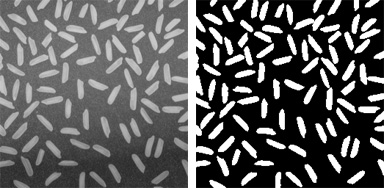
\includegraphics[width=\textwidth]{figures/segmentation0.jpg}
		\caption{\footnotesize \textbf{Binary Segmentation} \ \ \ \ \ A binary segmentation of rice.  We can use segmentation to create a binary mask that lets us separate the rice (foreground) from the darker background. \footnotemark[1]}
	\end{subfigure}
	~
	\begin{subfigure}[h]{0.45\textwidth}
		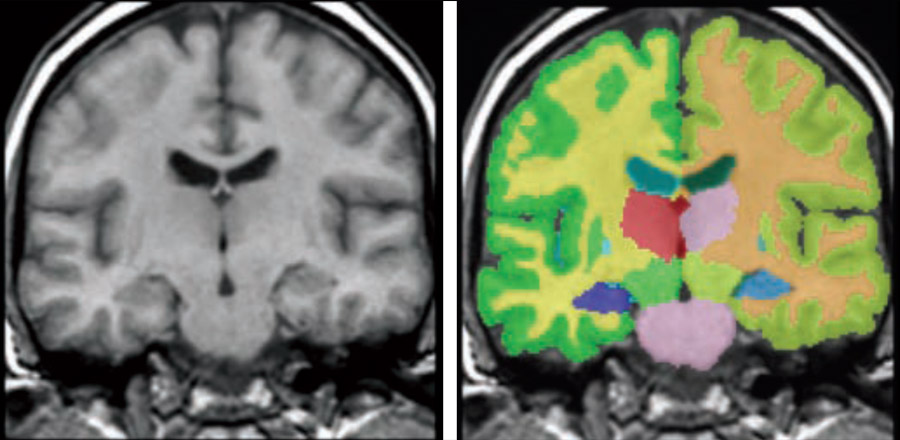
\includegraphics[width=\textwidth]{figures/segmentation1.jpg}
		\caption{\footnotesize \textbf{Multilabel Segmentation} \ \ \ \ \ A multilabel segmentation of a coronal section of a brain MR.  We can see that different colors represent different sections of the brain (left side white matter). \footnotemark[2]}
	\end{subfigure}
	\caption{Segmentation Example}
	\label{fig:segmentation}
\end{figure}\\
\footnotetext[1]{\texttt{http://www.mathworks.com/cmsimages/97744\_wm\_correcting-nonuniform-illumination.jpg}}
\footnotetext[2]{\texttt{http://www.bioclinica.com/sites/default/files/u1/atlas-based-brain-segmentation-lg.jpg}}
\indent A lot of radiological image analysis begins with segmentation.  For example, to quantitatively describe a lung nodule, you may want to collect data on its edge sharpness, it's total volume, or the mean intensity of voxels in the nodule.  However, to do this, we have to first be able to segment the nodule and cleanly define its boundaries.\\
\indent This can get extremely hairy.  For example, in the chest, it might be hard to teach a program to segment a nodule in the lung from a seed voxel, but it is important to make sure the nodule segmentation doesn't bleed into the pericardium, as the voxel intensities for a nodule and the fleshy bits in the pericardium are very similar.  Thus, we can define a region of interest where we limit our nodule segmentation to be within: this is lung field segmentation.  Basically, we want to go through our chest CT scans, and segment out the lungs.\\
\indent This assignment will help you understand many core concepts taught in the lectures and hopefully, integrate the lectures into a medically relevant application.  The goals of this project can include:
\begin{itemize}[noitemsep]
\item Understanding medical image data format, specifically, the \textbf{DICOM format}.
\item Understanding thresholding techniques, specifically, \textbf{Otsu's Threshold}.
\item Understanding \textbf{morphological image analysis} techniques, and expand this understanding into 3-D.
\item Understanding \textbf{image convolution}, and expanding it into efficient 3-D.
\item Understanding \textbf{visualizing 3-D}.
\item Embracing creativity and exploring image analysis.
\end{itemize}
\indent This can be a very daunting task for a first timer; however, I promise the final results will be amazingly cool!\\
\ \\














































\clearpage
\noindent \Large \textbf{Assignment Description} \normalsize \\
\noindent\makebox[\linewidth]{\rule{\textwidth}{0.4pt}}
\indent The main goal of this assignment is to segment the lung and only the lung from these CT slices, and then create a 3D rendering to give yourself some way to qualitatively assess how good your segmentation is.  Basically, given a chest CT series, we want you to produce
\begin{figure}[h]
	\centering
	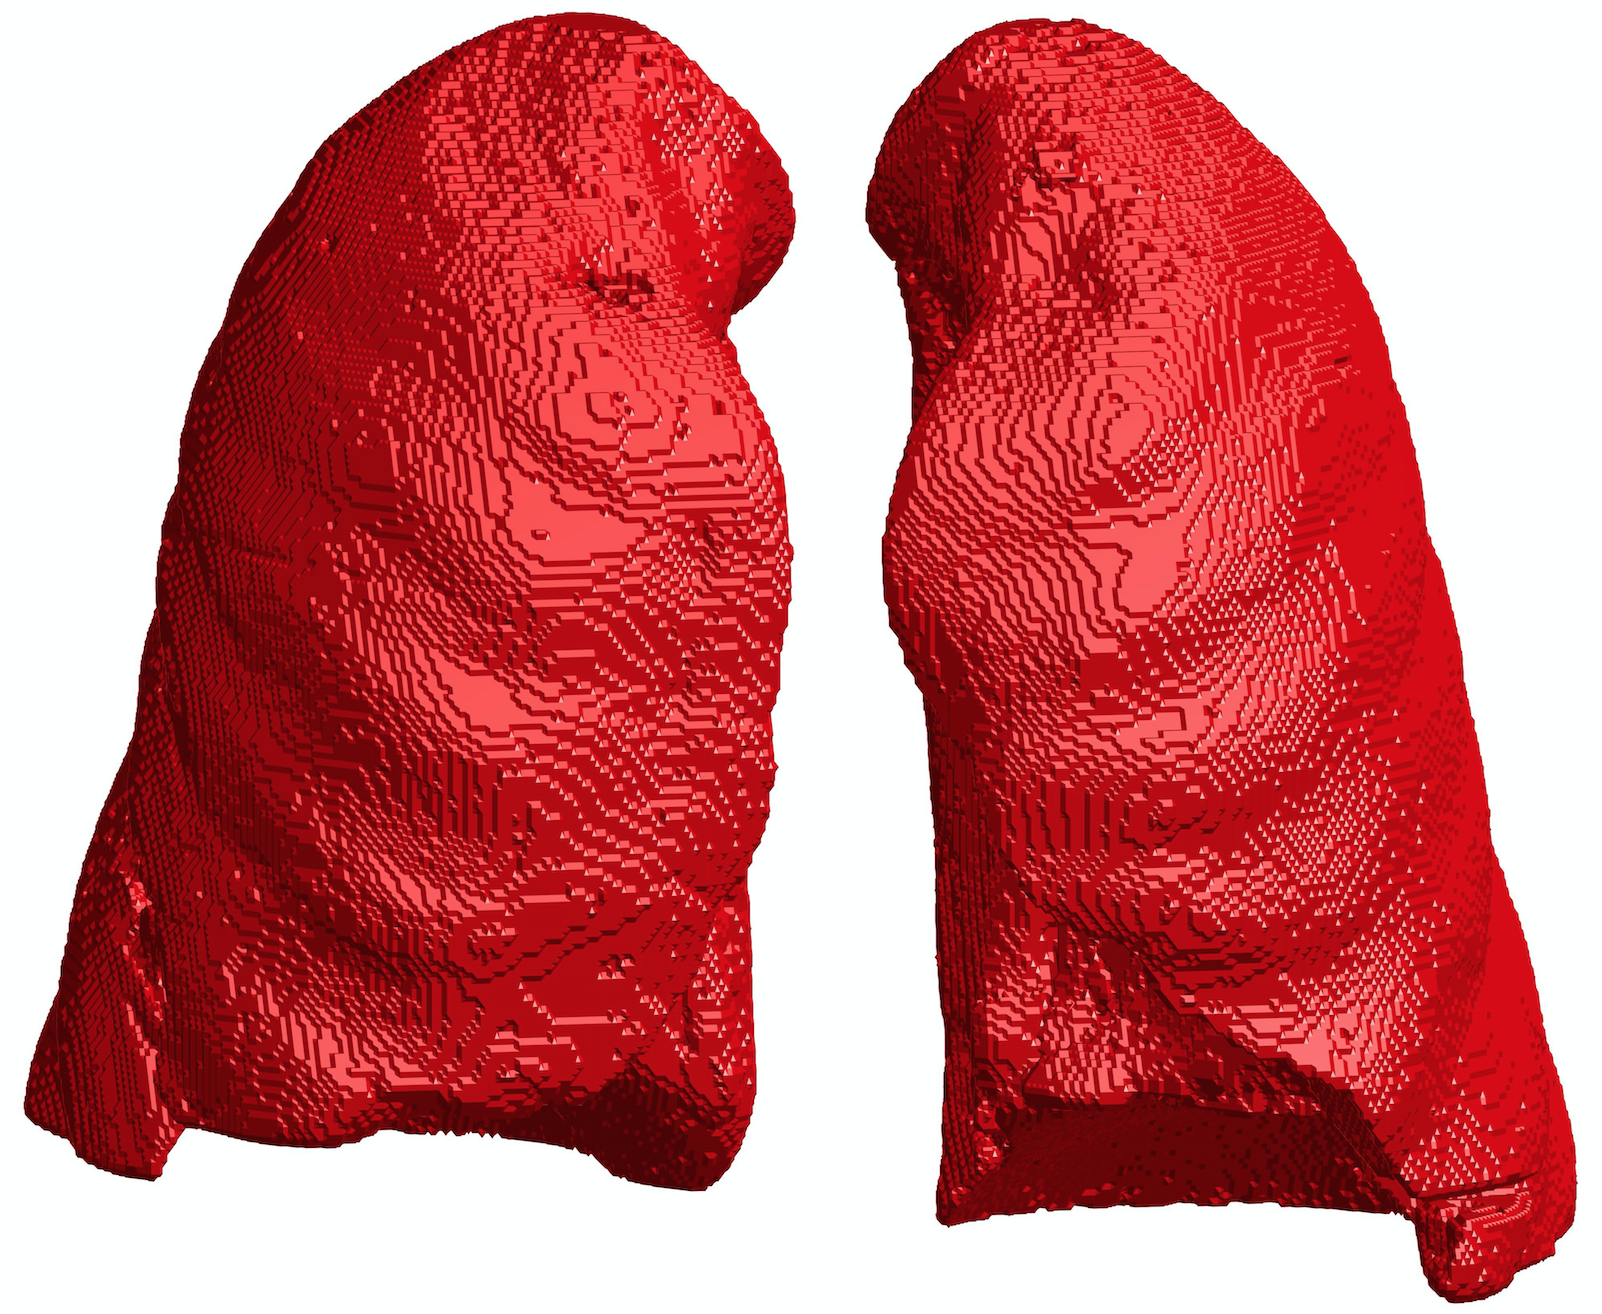
\includegraphics[width = 0.5\textwidth]{figures/lung_field_segmentation}
	\caption{Lung Field Segmentation 3D Rendering}
	\label{fig:LFS}
\end{figure}\\
What would be even better is if you could make a sort of movie that shows the full efficacy of your program to fully segment a lung.  You can find an example at \texttt{https://youtu.be/C8w92haDU24}.  However, that would be considered going above and beyond for the project, though it would teach you about the difficulties of rending and may give you a stronger appreciation for anything Pixar or Disney produces.\\
\indent This project is intended to be extremely open ended.  Below, I will give a detailed guideline of how I approached the Lung Field Segmentation problem, but at no point should you feel limited to solving the problem that way.  As long as you succeed in segmenting the lung and producing a 3D visualization of your result, you're golden.  Honestly, as long as you use the lungCT data provided in some way, you're more than free to even create your own assignment.  Do be warned, only do this if you are passionate about delving deeper into some aspect of this class and don't care too much about getting the perfect grade.  By turning the problem set into something in your own definition, you're making the grading process a full on conversation between you and us (the TA's).    Everything after this point is just recommendations and possibly implementations that you can use.  As soon as you have the data and a full understanding of what you have to do, you can start and finish the whole project without reading any more of this document after the ``submission description'' section.\\
\ \\
\ \\

\noindent \Large \textbf{The Data} \normalsize \\
\noindent\makebox[\linewidth]{\rule{\textwidth}{0.4pt}}
We will be using data from the recent (2017) Kaggle Data Bowl challenge.\footnote{https://www.kaggle.com/c/data-science-bowl-2017}  You can download their data freely.  I highly recommend downloading the ``sample\_images.7z'' file as they'll give you full CT scans, but won't take a day to download (total file $<$ 1gB)

The data is a series of sets of DICOM images that holds complete anonymized chest CT series (see section ``Reading in the Data'').
\textbf{Please download and unzip the data folder as soon as possible.}  Even the file for just the sample data is pretty big, coming in at $\sim$800mB.  You need the data to do the assignment.  We will not accept your using any other data.  Please try to download the data as soon as possible, and contact the TA's if you run into any problems.  \textbf{Do not wait until the last minute to download the data.}  For our collective sanity, just do this as soon as you read this section, yea?



















































\clearpage
\noindent \Large \textbf{Group Work} \normalsize \\
\noindent\makebox[\linewidth]{\rule{\textwidth}{0.4pt}}
You can work in groups of 2 without any change in how we'll grade your report.  If you're really endeavoring to do something grand, you can work in bigger groups.  However, with 3 or more people in a group, we'll expect you to have novel results at the level of an actual journal publication.  This scales with people.  With 4 people, I'm gonna expect a Nature level publication.  With 5, you better win a Nobel Prize.\\
\ \\








\noindent \Large \textbf{Submission Description} \normalsize \\
\noindent\makebox[\linewidth]{\rule{\textwidth}{0.4pt}}
\indent For this project, you will submit a .zip file containing everything you'd like to be considered for grading.  Please name it ``assignment1\_$\langle$suid1$\rangle$-$\langle$suid2$\rangle$.zip'' where you replace $\langle$suid1$\rangle$ with your actual Stanford University net id of the first person, $\langle$suid2$\rangle$ with the second person and so on.  Your .zip file should contain, but should not be limited to
\begin{itemize}[topsep=0pt,itemsep=-1ex,partopsep=1ex,parsep=1ex]
\item report\_$\langle$suid1$\rangle$-$\langle$suid2$\rangle$.pdf: The main publication camera-ready report showing off your findings and explaining your algorithm.  Format your report so that it follows some major journal/conference format.  Completely acceptable formats include MICCAI, IEEE, NIPs, and ICCV.  Other formats are valid too; you're free to roll the dice on that one.
\item \texttt{main.py} (\texttt{.sh}, \texttt{.m}, etc...): Some file we can run to produce the results detailed in your report.  All your dependencies should be called by this main file.  Your README.txt should give some detail as to how to run your programs.
\item \texttt{README.txt}: A general guide as to how we should run your code.  Also, if you added supplementary material, explain to us what it is and why you think its cool.
\item Code Dependencies
\item Supplementary Material: whatever else you want us to consider
\end{itemize}
Your total .zip file should be less than 20mB in size.  If your .pdf is large, consider putting it through some compressing program.  This is a hard limit.\\

\indent The assignment .pdf will follow the format of a submittable paper in a reputable journal/conference.  Thus, feel free to focus more on what you consider the more important aspects of what you discovered during the course of this assignment (i.e. following normal conventions of a paper, you don't/shouldn't focus on how you got to read in the DICOM format).  Completing the tasks outlined in the assignment alone will be enough to write a paper around; however, we highly encourage you to pursue one of the extra areas outlined below.  We are pursing a pure paper format for the submission reports for the following reasons:
\begin{itemize}[noitemsep]
\item thinking about the assignment as a submittable paper will help focus your work
\item writing an introduction will force you to do a literature review of what you're working on
\item problem sets suck and aren't applicable to life.  papers suck less.  get used to writing papers.
\item if you do indeed do something cool, you're ready to submit this right away, even if it's just to arXive.
\end{itemize}
\indent As for the grade, we will resort to the tasks outlined below as a rough backbone.  However, please do try to experiment more and explore this segmentation task or 3D data for more novel discovery without fear of falling behind in terms of the grade.  Highlight these extra novel contributions in your paper and we'll do our best to credit everything.\\
\indent Though the majority of your grade will be dependent on your .pdf, we will still take a close look at your program, and we will attempt running it.  Please make understanding your code as painless as possible via comments and your README.txt file.













































\clearpage
\noindent \Large \textbf{Reading in the Data} \normalsize \\
\noindent\makebox[\linewidth]{\rule{\textwidth}{0.4pt}}
Though this section is only worth 10\% of your total grade, it is arguably the most important part of the whole assignment.  I've found that 90\% of research is usually tedious tasks, such as figuring out the input/output of a certain file format.  However, this is extremely important as without I/O, you literally can not start analyzing the data.  \textbf{PLEASE START THIS EARLY.}  I know every TA for every class will tell you to start the assignment early, and I know the vast majority of you all will ignore this warning.  But if you could just finish just this section as soon as possible, you'll feel much better.  Trust me, nothing feels worse than being a few days away from the due date and not being able to read in the data.\\
\indent You will be working with Chest CT images.\footnote{We will use data from the most recent Kaggle challenge.}  The images are in DICOM format (``.dcm'').  You can find more information about this format in the DICOM standard.\footnote{http://dicom.nema.org/standard.html}  You can choose any of the patients in the Kaggle dataset (sample, training, or validation) to prototype your code, but we expect you to generalize your algorithm over at least 10 different patients to show robustness.  The more you do, the more you'll prove your algorithm.  Each file's data is made up of two parts: a header giving you a lot of information about the patient and specifics about the dataset (e.g. space between slices) and the main image portion.  We have previously mentioned that the assignment is very open-ended and you can use whatever method you find fittest to solve this problem.\\
\indent For python, we recommend using the \texttt{pydicom} package.\footnote{http://pydicom.readthedocs.io/en/stable/getting\_started.html}  Make sure you read the docs to find out how to read a dicom file (\textbf{HINT:} be sure to look up the API for \texttt{read\_file} and \texttt{pixel\_array}).  Be sure to take some time to print out your dicom object after reading a slice of your CT in.  For example, you should see something like this:\\
\begin{figure}[h]
	\centering
	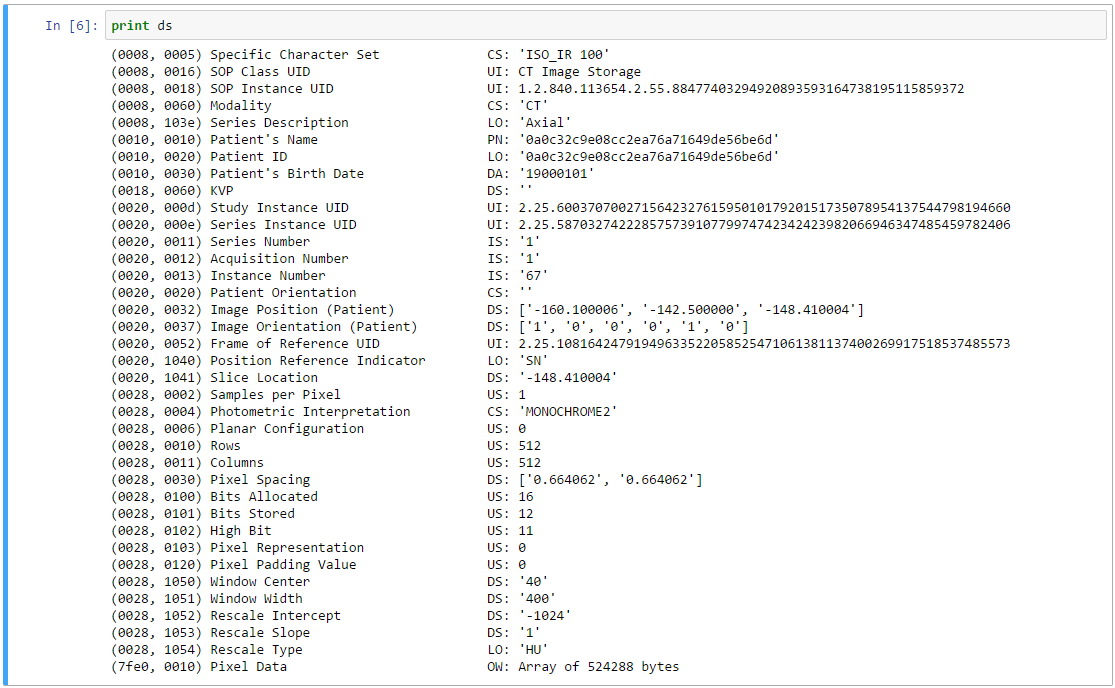
\includegraphics[width = 0.75\textwidth]{figures/dicom_fields}
	\caption{Dicom Fields}
	\label{fig:DCM}
\end{figure}\\
From figure \ref{fig:DCM}, we can see that there are many data fields in a dicom file.  There are many patient information stored in a dicom, such as patient's name and birth-date.  For obvious privacy reasons, this data has been completely anonymized as it's pretty evident that our data probably didn't come from Mr./Mrs. 0a0c32c9e08cc2ea76a71649de56be6d who was born on January 1st, 1900.  However, there are other important fields, such as rescale intercept or slope.  The default saved pixel values are some arbitrary units from the actual machine used.  However, as you learned in lecture, we'd like to use Houndsfield Units maybe, to have some standardization among all of our CT scans.  The conversion formula will be:
\begin{equation}\label{eq:HU}
\text{HoundsfieldUnits} = \text{RescaleSlope} * \text{Img} + \text{RescaleIntercept}
\end{equation}

\indent Once you use equation \ref{eq:HU} and the \texttt{pydicom} package to read in the image, you'll have to read in ALL the other images for a given CT scan.  The next main part of your problem will be to go from all the individual slices of the CT scan (each one stored as a .dcm file) into a 3D volume.  Basically, you'll need to figure out some way to order these slices in the right order.  Read in a few of the dicom images from your patient, and try using different dicom fields as a sorting key.  You may find one of them works well in sorting the slices in the correct order.  Try looking up what that field means in the dicom standard.  Visualize the volume you create from the stacks.  Feel free to do this within python with something like \texttt{matplotlib}, or use 3rd party software like Fiji (which is just imageJ).  If you ordered them correctly, you should get something like figure \ref{fig:order}.
\begin{figure}[h]
	\centering
	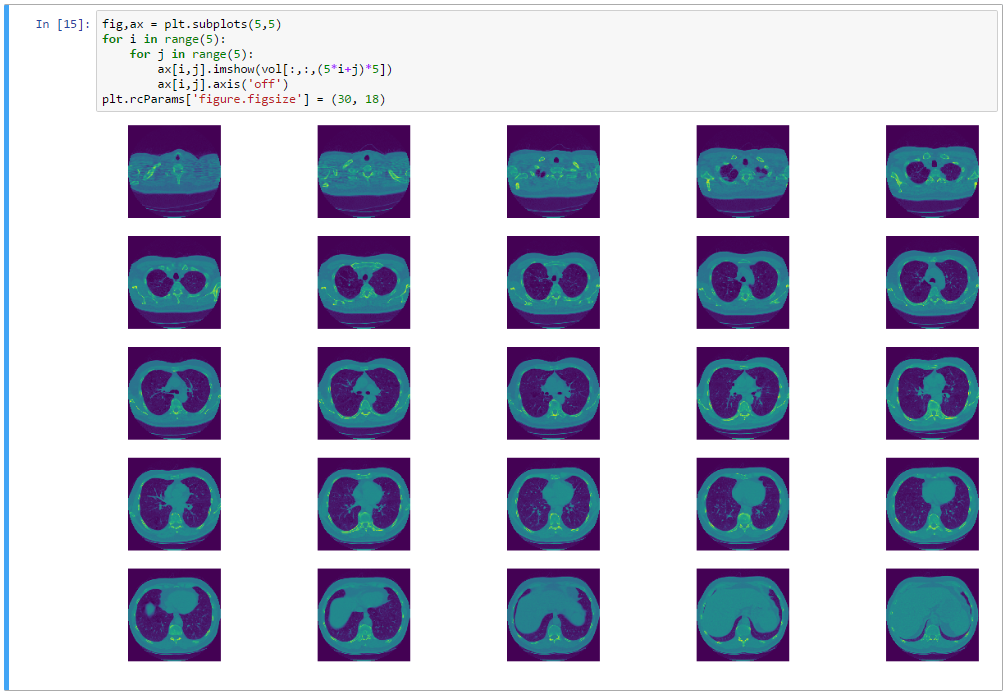
\includegraphics[width = 0.75\textwidth]{figures/lung_order}
	\caption{Slices Ordered}
	\label{fig:order}
\end{figure}\\

\indent To get the best visualization of the lung, think about what Houndsfield units mean.  You can see a general range in figure \ref{fig:HU}\footnote{http://www.odec.ca/projects/2007/kimj7j2/index\_files/Page1674.htm}.  Use this to maybe select the best range of pixel values to visualize.
\begin{figure}[h]
	\centering
	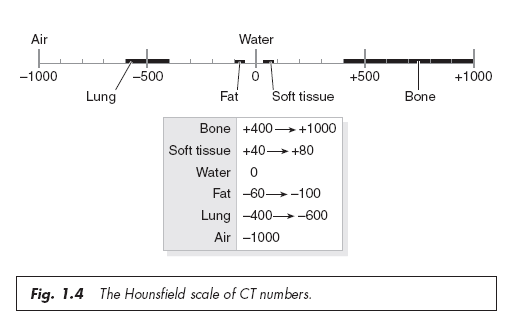
\includegraphics[width = 0.5\textwidth]{figures/houndsfield}
	\caption{Houndsfield Units}
	\label{fig:HU}
\end{figure}\\









































\clearpage
\noindent \Large \textbf{Segmentation: One Possible Approach} \normalsize \\
\noindent\makebox[\linewidth]{\rule{\textwidth}{0.4pt}}
\indent First, for the whole project, I considered everything to be in 3-dimensions.  Since your input data is technically in 3D, let's create a 3D matrix called \texttt{volCT}.  Here is some pseudo code for the logic:
\begin{center}
\begin{minipage}[c]{0.75\textwidth}
\noindent\makebox[\linewidth]{\rule{\textwidth}{0.4pt}}
\noindent \textbf{Algorithm 1: Creating Volume\\
Relevant Commands: \texttt{os.listdir}, \texttt{dicom.read\_file}, \texttt{numpy.zeros}, \texttt{numpy.shape}, \texttt{sort}}\\
\noindent\makebox[\linewidth]{\rule{\textwidth}{0.2pt}}
initialize \texttt{vol = }matrix of size \texttt{[\#pi$\text{x}_\text{width}$, \#pi$\text{x}_\text{height}$, \#slices]}\\
\texttt{for} each .dcm in folder:\\
\hspace*{1em} Read in .dcm\\
\hspace*{1em} Store number from header that acts as proxy for slice order.\\
\texttt{endfor}\\
\texttt{order} the saved numbers to index each DICOM file by slice order.\\
\texttt{for} each .dcm in folder:\\
\hspace*{1em} \texttt{s = }Slice Order of DICOM image\\
\hspace*{1em} Read in image as \texttt{img}\\
\hspace*{1em} \texttt{vol(:, :, s) = img;}\\
\texttt{endfor}\\
\noindent\makebox[\linewidth]{\rule{\textwidth}{0.2pt}}
\end{minipage}
\end{center}
You may also notice that our image is a 16-bit integer.  You may consider whether we want to keep our data that way?  Maybe we'd want to normalize our data somehow?\\
\indent Now that we have our 3D matrix of data, we can try to segment out our lung.  We know from lecture that CT scans work by Houndsfield Units, where lower intensities are for mediums where X-rays can pass through more easily, like air, and higher intensities are those that block the X-rays more, like bone.  Thus, you can see from histogramming the pixel values, we have quite the bimodal distribution.  And as we learned from class, we can find a nice separating value of our two modes with Otsu's method:
\begin{figure}[h]
	\centering
	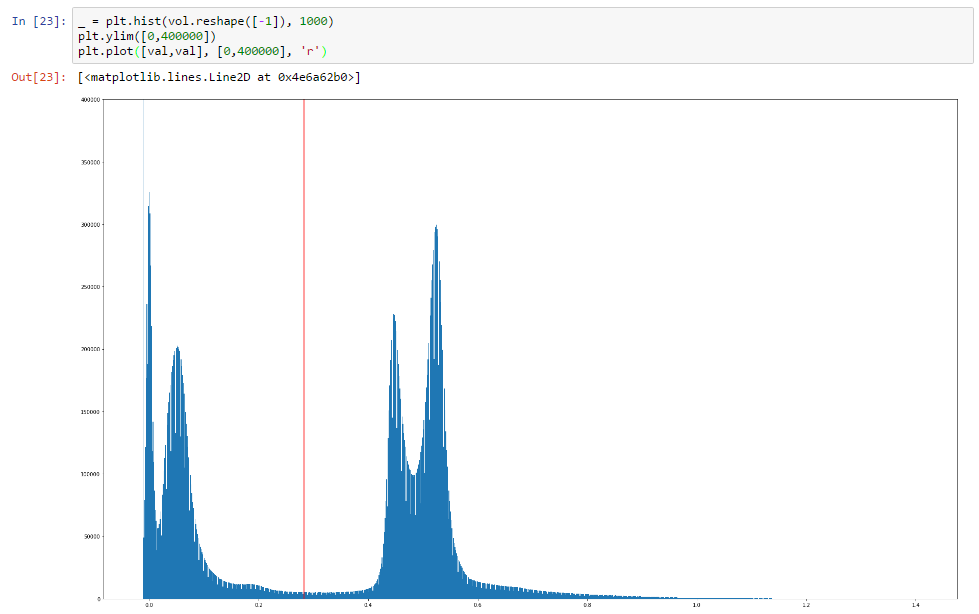
\includegraphics[width = 0.75\textwidth]{figures/histWithThresh}
	\caption{Histogram with Otsu's Threshold}
	\label{fig:otsu}
\end{figure}
\clearpage
\indent We can now take a look at what simple Otsu's threshold does.  We want to pick all the pixels less than Otsu's threshold since the lung is in the darker part of the image.  Thus,
\begin{figure}[h]
	\centering
	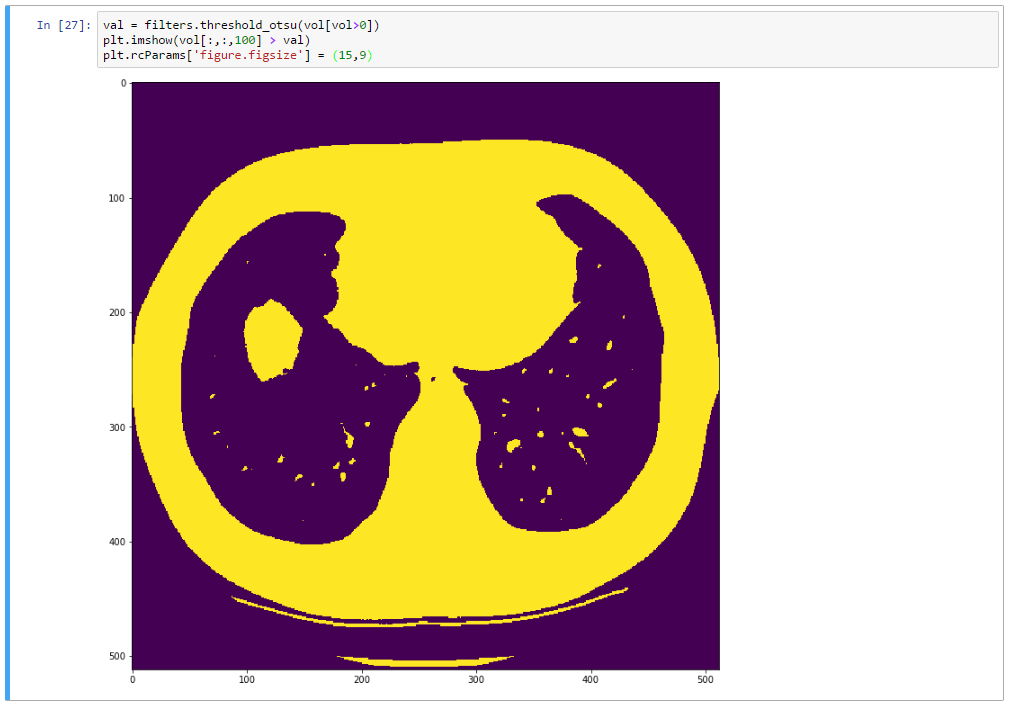
\includegraphics[width = 0.75\textwidth]{figures/otsu}
	\caption{Otsu's Method in Practice}
	\label{fig:otsu2}
\end{figure}
We can see that this is really close to what we want for a final result, but it's still a bit noisy.  Our dark lungs are surrounded by lighter colored flesh, which is then again surrounded by darkness.  However, this gives us a very interesting result.  Our lung segmentation is completely separated from segmentation of the outside.  These two sets of binary connected components are completely unconnected.  Thus, we can just filter out the outer segmentation by getting rid of any segmentation that is touching the outer most pixel.  Here would be a possible pseudo-code:
\begin{center}
\begin{minipage}[c]{0.75\textwidth}
\noindent\makebox[\linewidth]{\rule{\textwidth}{0.4pt}}
\noindent \textbf{Algorithm 2: Segmentation}\\
Relevant Commands: \texttt{skimage.filters.threshold\_otsu}, \texttt{skimage.measure.label}\\
\noindent\makebox[\linewidth]{\rule{\textwidth}{0.2pt}}
Find Otsu's threshold of \texttt{vol}, \texttt{thresh}.\\
Make binary volume mask of anything below \texttt{thresh}, \texttt{volBW}.\\
\texttt{for} each slice \texttt{s}:\\
\hspace*{1em} Find all binary connected components of slice \texttt{s}.\\
\hspace*{1em} \texttt{for} all connected components \texttt{i}:\\
\hspace*{2em} \texttt{if} connected component \texttt{i} touches the edge of the image:\\
\hspace*{3em} delete connected component \texttt{i}.\\
\hspace*{2em} \texttt{endif}\\
\hspace*{1em} \texttt{endfor}\\
\texttt{endfor}\\
\noindent\makebox[\linewidth]{\rule{\textwidth}{0.2pt}}
\end{minipage}
\end{center}

\indent However the segmentation's still rough around the edges.  There's a few pixels of noise around the main lung.  Components that weren't touching the edges, but still aren't part of the lung.  Luckily for us, these bits are quite small in size.  Thus, we can use a quick volume filter.  We want to choose connected components that have a volume greater than some threshold \texttt{V}.  You can choose this arbitrarily, as most noise will have pixel counts in the double digits or maybe low hundreds, but your lung volume should have a pixel count several orders of magnitude higher.
\begin{center}
\begin{minipage}[c]{0.75\textwidth}
\noindent\makebox[\linewidth]{\rule{\textwidth}{0.4pt}}
\noindent \textbf{Algorithm 3: Volume Filter}\\
\noindent\makebox[\linewidth]{\rule{\textwidth}{0.2pt}}
Find all the 3D connected components in your \texttt{volBW}.\\
\texttt{for} each connected component \texttt{i}:\\
\hspace*{1em} \texttt{if} connected component's volume $<$ \texttt{V}:\\
\hspace*{2em} Delete Connected Component \texttt{i}.\\
\hspace*{1em} \texttt{endif}\\
\texttt{endfor}\\
\noindent\makebox[\linewidth]{\rule{\textwidth}{0.2pt}}
\end{minipage}
\end{center}
\ \\
\indent After this, we just want to smooth out the edges.  The segmentation of our lung looks very ragged because it wasn't able to pick out the lighter colored blood vessels in the lung.  Thus, we can do this with the image close algorithm.  Luckily for us, \texttt{scikit-image} has already programmed the image close algorithm, \texttt{skimage.morphology.binary\_closing}, which works for both 2-dimensional and 3-dimensional binary matrices.
\ \\
\ \\
\ \\
\ \\
\textbf{Above and Beyond:}  If you've finished everything above, you've already done a full fledged segmentation.  However, for an extra challenge, you can try your hand at removing just the trachea so that your segmentation is just on the left and right lung without any of the trachea or bronchi.  It would be great to see if you can separate out the two halfs of the lung into left/right lungs.  This would be a much more clinically useful algorithm as well.










































\clearpage
\noindent \Large \textbf{Visualization} \normalsize \\
\noindent\makebox[\linewidth]{\rule{\textwidth}{0.4pt}}
\indent To really showcase your results, you should add some sort of visualization to your report in the Results section.  We recommend showcasing both 2 and 3 dimensional visualization.  Showing 2-dimensional results in the form of an array of slices gives a more detailed view of your segmentation.  The 3-dimensional result is just a sexier visualization, and makes your paper look more professional.\\
\indent The simplest way to visualize your segmentation in 3D would be to create a 3D scatter plot where you have a point per $[x,y,z]$ point where you have a segmented lung pixel.  This will still bag you some of the points, should you not want to go on to the full 3D rendering, but it's just not as elegant.\\
\indent A better way might be to use some 3rd party visualization software.  There are a ton of python packages that can do this, but it might be a difficult to grasp.  We highly recommend looking up some marching cube algorithms, but the easier way to go would probably use something like Fiji.\footnote{https://fiji.sc/}  Simply download Fiji (available for Windows, Mac, and Linux).  You can save all your 3D segmentation as binary image slices.  Then, using Fiji, simply read in your image sequence (be sure to name your images some numeric count or something so that Fiji knows what order to read the images in).  Then, go to $>$plugins$>$3D Viewer.  This should give you a figure like what you see below.
\begin{figure}[h]
	\centering
	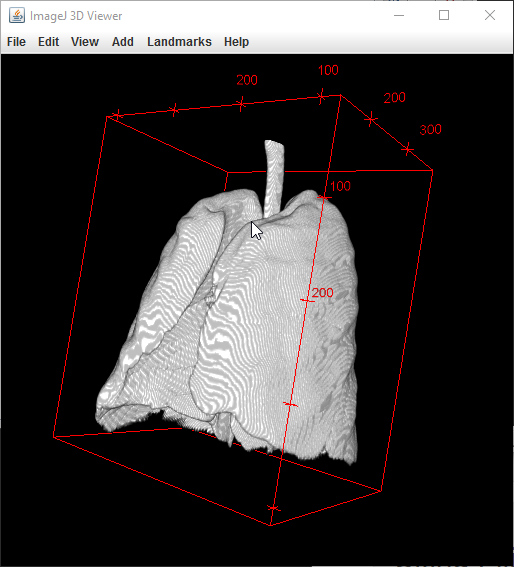
\includegraphics[width = 0.67\textwidth]{figures/3d_vis}
	\caption{3D Visualization: Scatter Plot and Rendering}
	\label{fig:visualization}
\end{figure}

\indent The main goal of visualization (in my opinion) is to help us understand how our algorithm succeeded and failed.  Thus, using your visualization (if you didn't get any of the 3D visualization to work, just respond to a 2D visualization), explain how your algorithm worked.  Acknowledge both the good and bad of your algorithm.  If there's only good, good on you, but you better be sure your work can back up your hubris.\\
\ \\












































\clearpage
\noindent \Large \textbf{Validation} \normalsize \\
\noindent\makebox[\linewidth]{\rule{\textwidth}{0.4pt}}
Since we're looking at the Data Bowl, you have more than a thousand lung CT's to play around with.  Make sure you run your algorithm on several more lungs and try to come up with a clear visualization method that maybe shows summary results for a representative chunk of lungs.






































\clearpage
\noindent \Large \textbf{Grading Rubric} \normalsize \\
\noindent\makebox[\linewidth]{\rule{\textwidth}{0.4pt}}
\begin{table}[h]
 \caption{\textbf{Grading Rubric} \small{As stated in multiple places in this problem set, this rubric is only meant for your defense.  We can be much more generous with the rubric.  This rubric should just be used as a general guide to ensure that you have some goal.}}\label{table:Comparison}
\begin{center}
\begin{tabular}{L{2.5cm}|L{9cm}|L{2cm}}
\toprule[1.5pt]
Section & Description & Percentage \\
\midrule
\midrule
Title & Choose a good title that is concise, clear, and fully demonstrates the problem you are attempting to solve. & 5\\
Abstract & A proper scientific abstract that discusses
	\vspace{-3mm}
	\begin{itemize}[noitemsep]
	\item the general problem to be solved (2)
    \item the main contribution to science (2)
    \item the summary results (1).
	\end{itemize}& 5\\
Introduction & This will mainly deal with doing some literature research. This is an extremely loose rule of thumb, but aim to have maybe 10 citations in this section.  We want to see
	\vspace{-3mm}
    \begin{itemize}[noitemsep]
    \item background research on the problem (10)
    \item background research on other solutions (10)
    \item background information on your methods (5)
    \end{itemize}& 25\\
Dataset & Talk about the dataset that you are using. Give some background on where the data came from and let the reader understand what the data your using is.  Cite the data source. & 10 \\
Methods & Explain the approach you used. You don't have to go into too much of the detail if the detail is trivial.  You can assume the general knowledge of the field you're writing your scientific paper to. & 15 \\
Results & Showcase your results.  This is a very visual project.  Figure out a way to create a wonderful figure that really proves that you've accomplished what you want to create. & 15\\
Discussion & Discuss your algorithm.  Tell us where it stands within the current field.  What value have you added to the medical imaging community.  Finally, make sure you do talk about the limitations of your research.  Nothing is worse than overstating your results.  This really is a tightrope walk.  You want to showcase how sexy your results are, but you don't want to overstate them either.  Good luck. & 20\\
Style & Basically, aim to write well and keep all your code clean.  If you do switch off writing some sections, make sure that the voices between sections don't clash in a jarring way. & 5\\
\midrule
\midrule
\end{tabular}
\end{center}
\end{table}


\ \\
\textbf{NOTE:} Again, the above is a proposed rubric for what I (Darvin) think is a good scientific paper.  The main requirement is that you write a mock-paper (in any reputable journal).  There are different theories on how papers should be formatted and what should go in each section.  If you have a preferred style, do whatever you want.  Obviously, some parts of the rubric (e.g. the title, abstract, and introduction) are a bit more standard, but format the rest however you want.  We're really not trying to trap or hurt you here.









































\clearpage
\noindent \Large \textbf{Frequently Asked Questions} \normalsize \\
\noindent\makebox[\linewidth]{\rule{\textwidth}{0.4pt}}
\begin{itemize}[noitemsep]
\item \textbf{How does grading work?} \ \ \ \ \ \ \ \ \ \ \textit{Don't worry about grading so much.}  But I know you will.  If getting or securing that perfect hw score is an important thing in the world to you, just do the minimal tasks outlined in this problem set and showcase your segmentation results together with your pipeline and focus on the write-up as a minimum, since you can use that to defend why you deserve full credit later on.
\item \textbf{Is ----- a good addition/substitution to the assignment?} \ \ \ \ \ \ \ \ \ \ Ask on piazza.
\item \textbf{Do I have to use \LaTeX?} \ \ \ \ \ \ \ \ \ \ \textit{No.}  You just have to use the style of a reputable journal/conference.  Many journals/conferences have templates in word or whatever.  Just submit a .pdf (i.e. print to pdf).  We don't want to deal with figures being out of place.
\item \textbf{Is ----- a reputable journal/conference?} \ \ \ \ \ \ \ \ \ \ Ask on Piazza.
\item \textbf{Access to computational resources?} \ \ \ \ \ \ \ \ \ \ The current assignment should be able to be done on a simple computer or the shared Stanford resource of \texttt{corn.stanford.edu}.  If you are attempting to do something on a grander scale and would like additional computational resources, please contact the TA's.  We have some cloud computing credits we are reserving for projects and future assignments as well as lab resources that we could possibly support you with.
\item \textbf{Do we have late days?} \ \ \ \ \ \ \ \ \ \ \textit{No.}  You're an adult.  Submit your stuff on time or fail gracefully.
\item \textbf{What if my computer froze last minute, and that's why my assignment's late.} \ \ \ \ \ \ \ \ \ \ \textit{Don't do this.}  We'll only grade the most recently submitted .zip file after the assignment is due, so just submit your assignments often.  Aim to submit your assignments at 9pm instead of midnight to give yourself a 3hr grace period in case of computer troubles.
\item \textbf{What if I go through an emergency?} \ \ \ \ \ \ \ \ \ \ Obviously, that's different.  Contact the TA's privately via email or Piazza for extensions.  Life happens.  we understand that and by no means want to make your life worse.

\end{itemize}






\end{document}